\section{生命游戏与元胞自动机}

\subsection{生命游戏}

\begin{figure}[htb]
	\centering
	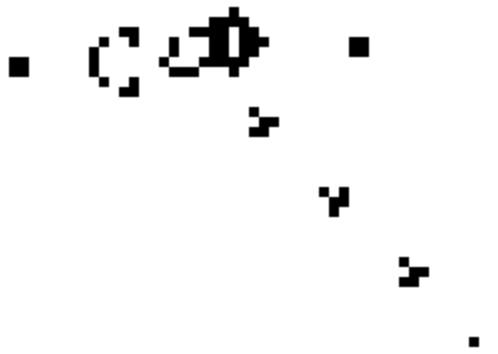
\includegraphics[width=2in]{figure/ConwayGame/Gospers_glider_gun.png}
	\caption{生命游戏的一种模式--高斯帕机枪}\label{fig_4.1}
\end{figure}


\subsubsection{定义与规则}

生命游戏的全称为\emph{康威生命游戏(Conway's Game of Life)},是由英国科学家John Horton Conway于1970年发明的一种元胞自动机。游戏中我们所看到的每一个方格我们称之为\emph{细胞},每个细胞有两种状态,\emph{存活}以及\emph{死亡}。每个细胞的存活状态由周围的八个方格内的细胞状态所决定,其具体的规则如下\cite{cgame:1}:

\begin{enumerate}
    \item \emph{活细胞}的周围有~{\color{red}\emph{2}}~或~{\color{red}\emph{3}}~个活细胞,则细胞会在下一轮\emph{存活}。
    \item \emph{活细胞}的周围的活细胞\emph{小于}~{\color{red}\emph{2}}~个的时候($<2$),细胞会在下一轮\emph{死亡}。
    \item \emph{活细胞}的周围的活细胞\emph{大于}~{\color{red}\emph{3}}~个的时候($>3$),细胞会在下一轮\emph{死亡}。
    \item \emph{死细胞}的周围的活细胞正好\emph{等于}~{\color{red}\emph{3}}~个的时候($=3$),这个死细胞会在下一轮\emph{存活}。
\end{enumerate}

以最初的细胞状态定义为初始态的\emph{种子},对这个状态下的所有细胞\emph{同时}进行上述的规则判断并进行变换,得到了下一轮的状态图。如此周而复始,生命游戏便不断的进行下去。

上述的规则用比较通俗易懂的话来解释一下的话,就是规则1像是模拟了正常的生存环境;规则2像是模拟了周围的资源过少;规则3像是模拟了周围资源竞争的压力过大;规则4则像是模拟了正常的繁殖环境。



% 参考文献
\bibliographystyle{unsrt}
\begin{thebibliography}{}
    \bibitem{cgame:1}
    Wikipedia--康威生命游戏, 
    \url{https://zh.wikipedia.org/wiki/%E5%BA%B7%E5%A8%81%E7%94%9F%E5%91%BD%E6%B8%B8%E6%88%8F}
    \bibitem{cgame:2}
    LifeWiki, \url{https://www.conwaylife.com/wiki/Main_Page}
\end{thebibliography}
